\section{Multi-Fingered Grasping}
\label{sec:multifingered_grasping}

A multi-fingered grasping is realised over a set of contacts between the active pairs (the workpiece and the gripper). Therefore, the determination of a suitable configuration of independent grasping points is the primary step of the fingered grasping planning. 

The wrench vectors describe the forces and moments that influence a rigid body's dynamic. These vectors can be used to formulate grasping locations, and a wrench vector is presented below:  

\begin{equation}
\mathbf{w_{c}}=\left[\begin{array}{l}
\mathbf{f} \\
\boldsymbol{\tau}
\end{array}\right]
\end{equation}

\noindent
where $\mathbf{f}$ and $\boldsymbol{\tau}$ are the column vector representations of the forces and the moments. The wrench vectors have 3 and 6 \acp{DOF} in the case of $\mathbb{R}^2$ and $\mathbb{R}^3$, respectively.

The contact models can be categorised as friction-less contact, friction contact (also named hard finger contact), and soft contact~\cite{murray1994mathematical}. The focus of this chapter will be the friction contact, since this model covers the main application field of this thesis.

%The friction contact model considers the mechanical interaction between the active pairs. Therefore, the wrench convex depends on the friction contact forces, described by Coulomb model of friction: Considering the normal force $\mathbf{f_n}$, and the tangential force $\mathbf{f_t}$, static friction occurs when there is no slipping between the two surfaces of contact, that is when $\left|\mathbf{f_{t}}\right| \leq \mu_{t} |\mathbf{f_{n}}|
%$ where $\mu_{t} $ is a positive value representing the static tangential coefficient of friction. Figure~\ref{fig:friction_contact} shows an example of hard finger contact, the geometric representation of the Coulomb’s law and the friction cone convex also defined as ${FC}_{c_i}$. 

The friction contact model considers the mechanical interaction between the active pairs which is defined by Coulomb model of friction. In this modelling, considering the normal force $\mathbf{f_n}$, and the tangential force $\mathbf{f_t}$, static friction occurs when there is no slipping between the two surfaces of contact, that is when $\left|\mathbf{f_{t}}\right| \leq \mu_{t} |\mathbf{f_{n}}|
$ where $\mu_{t} $ is a positive value representing the static tangential coefficient of friction. Figure~\ref{fig:friction_contact_model} shows an example of hard finger contact with its geometric representation of the Coulomb’s law and the friction cone convex ${FC}_{c_i}$. 

\begin{figure}[h!]
\resizebox{0.75\textwidth}{!}{%
\begin{tcolorbox}
\centerline{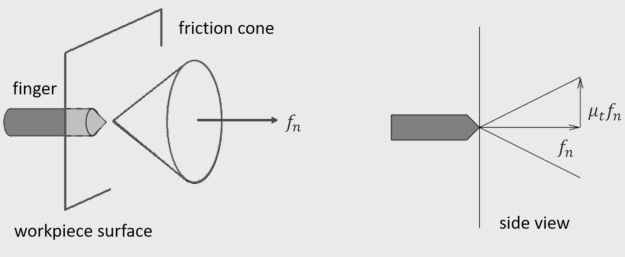
\includegraphics[trim={0cm 0cm 0cm 0cm},clip,width=1\linewidth,angle=0]{Apendices/Figuras/friction_contact_gray_bg2.pdf}}
\end{tcolorbox}
\caption{Friction contact model and the geometric representation of Coulomb’s law (figure based on~\cite{murray1994mathematical}).}
\label{fig:friction_contact_model}
} %end resize box
\end{figure}

It is important to note that in this model any torque ($\boldsymbol{\tau}_{c_{i}}$) is considered, i.e. $\boldsymbol{w}_{c_{i}} = \mathbf{f}_{c_i} \quad | \quad \mathbf{f}_{c_i} = [f_x, f_y, f_z]'$. Therefore, a tridimensional wrench hard finger representation, w.r.t the $i$-th contact point ($c_i$) could be defined as follows:

\begin{equation}
\mathbf{W_{c_i}}=\begin{bmatrix}
1 & 0 & 0 \\ 
0 & 1 & 0 \\ 
0 & 0 & 1 \\ 
0 & 0 & 0 \\ 
0 & 0 & 0 \\ 
0 & 0 & 0 
\end{bmatrix} \mathbf{f}_{c_i}, \quad \mathbf{f}_{c_i} \in F C_{c_i}
\end{equation}

\noindent
where $F C_{c_i}=\mathbf{f} \in \!R^3: \sqrt{f_{x}^{2}+f_{y}^{2}} \leq \mu_{t} f_{z,}, f_{z} \geq 0$, and $\mu_t$ is the transversal friction coefficient in $c_i$. 

Therefore, based on this wrench representation, it is possible to define the matrix that compose the wrench vector concept:

\begin{equation}
\mathbf{W}_{c_i}=\mathbf{B}_{c_i} \mathbf{f}_{c_i}, \quad \mathbf{f}_{c_i} \in F C_{c_i}
\end{equation}

\noindent
where $\mathbf{{B}_{c_i}}$ is the wrench basis matrix with dimension $p \times n$ where $p$ is the \acp{DOF} and $n$ the number of independent forces that constitutes $\mathbf{{f}_{c_i}}$, i.e. that is applied in the contact model. The contact model discussed here has as reference frame the one with the origin coincident with the contact point itself. It is more convenient to refer all contacts in a grasp model to a common frame, generally the centre of mass of the work piece. Therefore the wrench transformation matrix is defined as follows:

\begin{equation}
^{o} \mathbf{Tw}_{c_i}=\left[\begin{array}{cc}
{^{o} \mathbf{R}_{\mathrm{c_i}}} & {0} \\
{^o \widehat{\mathbf{t}}_{\mathrm{c_i}} {}^{o} \mathbf{R}_{\mathrm{c_i}}} & {^{o} \mathbf{R}_{\mathrm{c_i}}}
\end{array}\right]
\in \mathbb{R}^3
\end{equation}

\noindent
where $ ^o\mathbf{R}_{c_i}$ and $^o\mathbf{t}_{c_i}$ are the rotation and translation matrix of the $i$-th contact point ($c_i$) w.r.t. object frame ($o$). The $^o \hat{\mathbf{t}}_{\mathrm{c_i}} {}^{o} \mathbf{R}_{\mathrm{c_i}}$ is the skew-symmetric representation of the cross product $^o\mathbf{t}_{c_i} \times {{{}^o}\mathbf{R}}_{c_i}$ in format of the Equation~\ref{eq:operator1}.% presents an example of the referred operator to a generic tridimensional vector $\boldsymbol{a}$.

%\begin{equation}
%\widehat{\boldsymbol{t}}=\left[\begin{array}{ccc}
%0 & -a_{3} & a_{2} \\
%a_{3} & 0 & -a_{1} \\
%-a_{2} & a_{1} & 0
%\end{array}\right] \quad where \quad \boldsymbol{a} = \left[\begin{array}{c}
%a_{1} \\
%a_{2} \\
%a_{3}
%\end{array}\right]
%\label{eq:operator1}
%\end{equation}

\begin{equation}
^o \hat{\mathbf{t}}_{\mathrm{c_i}} {}^{o} \mathbf{R}_{\mathrm{c_i}}=\left[\begin{array}{ccc}
	0 & -x & y \\
	z & 0 & -x \\
	-y & x & 0
	\end{array}\right] \mathbf{R}_{\mathrm{c_i}}
	\label{eq:operator1}
	\end{equation}


Hence, the contact map $\mathbf{G}_{i}$ is defined as follows:

\begin{equation}
\mathbf{G}_{i}=^{o} \mathbf{T} \mathbf{w}_{c_i}^{\prime} \mathbf{B}_{c_i}
\end{equation}

Note that it describes the direction of each component of the $i$-th applied wrench and defines the constraints of the contact. The grasp map is the matrix with all contact maps that characterise the contact model (it is also named constraint matrix):

\begin{equation}
\mathbf{G}=\left[\begin{array}{llll}
{{}^o \mathbf{T} \mathbf{w}_{c_1}^{\prime} \mathbf{B}_{c_1}} & {\dots} & {{}^{o} \mathbf{T} \mathbf{w}_{c_N}^{\prime} \mathbf{B}_{c_N}}
\end{array}\right]
\end{equation}

Then, including the magnitude of the forces, a workpiece wrench can be written:

\begin{equation}
^{o} \mathbf{W}=\left[\mathbf{G}_{1}, \ldots, \mathbf{G}_{N}\right]\left[\mathbf{f}_{c_1}^{\prime}, \ldots, \mathbf{f}_{c_N}^{\prime}\right]^{\prime}=\mathbf{G} \mathbf{F}
\end{equation}

\noindent
where: $\mathbf{F} \in F C \text { and } F C=F C_{c_1} \times \ldots \times F C_{C_N}$

The grasp map is an important matrix since it is the mathematical formulation of a multi-finger grasping. From now on, the common reference frame is defined as the object frame, and for convenience, the $^{o}\mathbf{W}$ will be substituted by $\mathbf{W}$. Each column of $\mathbf{W}$ represents the independent contact wrenches. All the contacts discussed here are punctual contacts since the other kinds of contact can be approximate by a set of punctual contacts and edge contacts.

By means of the convex linearisation of the friction contact, Figure~\ref{fig:friction_contact_linearised}, it is possible to represent the contact force ($\mathbf{f}_{c_i}$) as a linear combination of the cone edges ($\mathbf{s}_{c_i}$ = $[s_x,s_y,s_x]'$) and ($a_d$):

\begin{figure}[h!]
	\resizebox{0.75\textwidth}{!}{%
		\begin{tcolorbox}
			\centerline{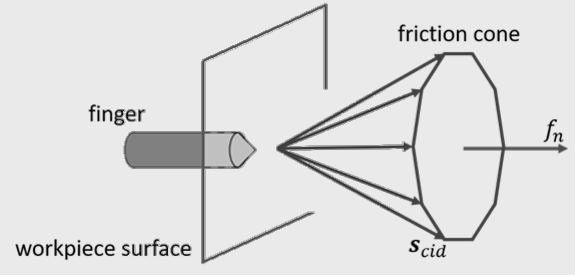
\includegraphics[trim={0cm 0cm 0cm 0cm},clip,width=1\linewidth,angle=0]{Apendices/Figuras/friction_contact_linearised.pdf}}
		\end{tcolorbox}
		\caption{Linearised friction contact model.}
		\label{fig:friction_contact_linearised}
	} %end resize box
\end{figure}


\begin{equation}
	\mathbf{f}_{ci} \approx \sum_{d=0}^{D} a_{d} \mathbf{s}_{ci_d}, a_{d} \geq 0 \quad, \quad \sum_{d=0}^{D} a_{d}=1
\end{equation}

where D is the number of edges that composes the linearised cone. A matrix notation can be formed as:

\begin{equation}
	\mathbf{f}_{ci}=\mathbf{A} \mathbf{S}_{ci}^{\prime}
\end{equation}

with $\mathbf{A}=\left[a_{0}, \ldots, a_{D}\right]$ and $\mathbf{S}_{ci}=\left[\mathbf{s}_{ci_0}, \ldots, \mathbf{s}_{ci_D}\right]$

Therefore, including all contact forces, the $\mathbf{W}$ associate with $\mathbf{S}$ is called primitive grasp map, also referred as primitive wrench map, defined as follow:

\begin{equation}
	\mathbf{W}_{p}=\left[\mathbf{G}_{1}, \ldots, \mathbf{G}_{N}\right]\left[\mathbf{A} \mathbf{S}_{c 1}^{\prime}, \ldots, \mathbf{A} \mathbf{S}_{c N}^{\prime}\right]^{\prime}=\mathbf{G} \mathbf{F}_{\mathbf{p}}
\end{equation}

The columns of $\mathbf{W}_{p}$ represent all wrenches associated with the edges of the linearised friction cone of the N contacts. It is an interesting matrix since it defines boundary conditions of contact. Applying a torque factor $\alpha$ (ensuring $|\tau| \leq|F|$) in each $w_{pd_{ci}}$ in $\mathbf{W}_{p}$, i.e.:

\begin{equation}
	w_{c}=\left[\begin{array}{c}
		\boldsymbol{f} \\
		\alpha \boldsymbol{\tau}
	\end{array}\right]
\end{equation}

and defining $\alpha=\frac{1}{r}$, where $r$ is the maximum radius of the centre of mass or gravity of the object and a contact point, it is possible to evaluate the grasps independently of the object size.

The $\mathbf{W}_p$ of all contact forces also defines the GWS (grasp wrench space) of the grasping. It is obtained by means of the $L_\infty$ or $L_1$ norm over the vector $\mathbf{g}$ composed by the magnitude of each contact normal force. The $L_\infty$ defines the GWS($W_L\infty$) considering the limitation of the maximum allowable normal contact force, while $L_1$ defines the GWS($W_{L1}$) by the sum magnitude of the normal contact forces. The norms operation yields to:


\begin{equation}
\begin{aligned}
\mathbf{W}_{L_{1}} &=\text { ConvexHull }\left(\bigcup_{c_i}^{N} \mathbf{w}_{p_1 c_i}, \ldots, \mathbf{w}_{p D_{c_i}}\right) \\
\mathbf{W}_{L_{\infty}} &=\text { ConvexHull }\left(\bigoplus_{c i}\left\{\mathbf{w}_{p_1 c_i}, \ldots, \mathbf{w}_{p D_{c_i}}\right\}\right)
\end{aligned}
\end{equation}

\noindent
where $\mathbf{w}_{pd_{ci}}$ $\in$ $\mathbf{W}$ and $\bigoplus$ is the Minkowski sum. More detail about the norm operation can be verified in~\cite{Ferrari}.


The concept of grasp closure evaluates the restraining of an object. A common assumption is the force-closure implies an equilibrium, but the inverse does not apply. A grasp has its convex hull defined by the wrenches that constitute the grasp configuration, i.e., the matrix $\mathbf{W}$. In a force-closure grasp, the convex hull includes the wrench space origin $\{O\}$, see Figure~\ref{fig:gws_force_closure}. According to the definition presented in~\cite{salisbury1983kinematic}, if all wrenches in $\mathbf{W}$ positively span the entire wrench space, the grasp will be force-closure. Figure~\ref{fig:gws_force_closure} shows a  grasp wrench space (GWS) and a convex hull of grasp configuration for force and non-force-closure, for a planar case with a fixed value for the moment ($\tau$) in the z-axis. Therefore, it is considered $\mathbf{f}_{c_i} \in  \mathbb{R}^2:  {f}_{c_i}  = (f_{x} , f_{y})$, and  the resistance to perturbation in both force axes is evaluated. 

\begin{figure}[h!]
\resizebox{0.8\textwidth}{!}{%
\begin{tcolorbox}
\centerline{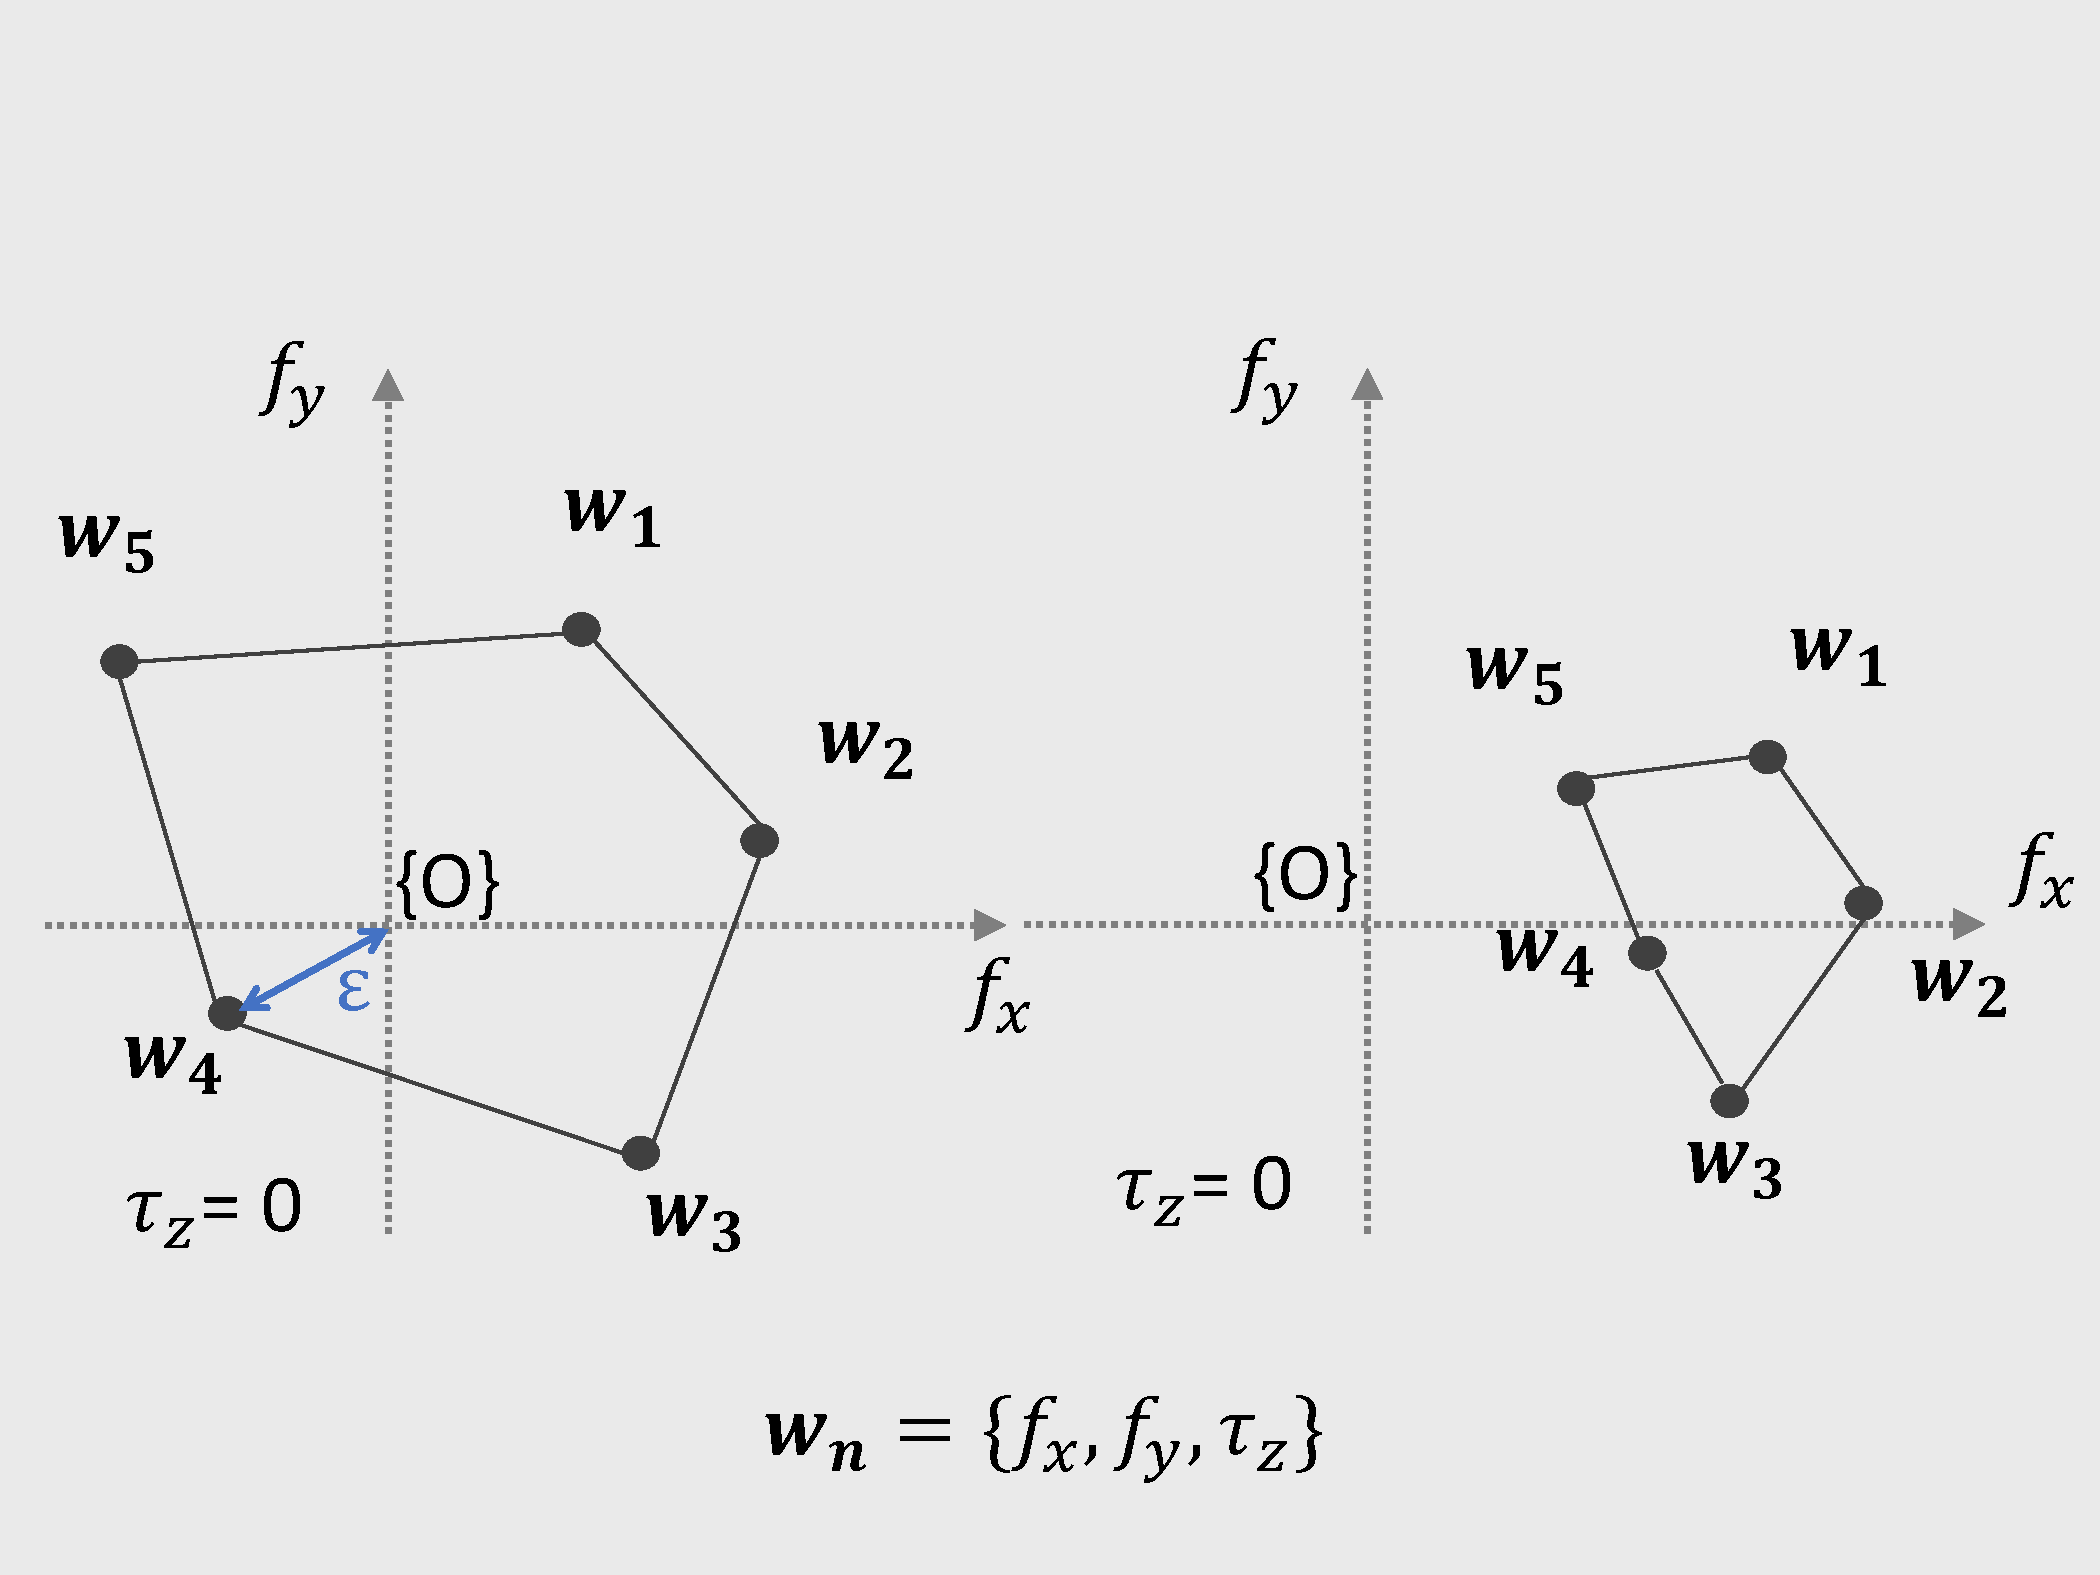
\includegraphics[trim={0cm 1.2cm 0cm 5.5cm},clip,width=1\linewidth,angle=0]{Cap2/Figuras/wrenchspace_anlayses_2.pdf}}
\end{tcolorbox}
\caption{Wrench convex-hull configuration. Force-closure and the $\epsilon$-value (left). Non-force-closure (right).}
\label{fig:gws_force_closure}
}%end resize box
\end{figure}

Since several configurations can reach a force-closure grasp, quality metrics like $\epsilon$-metric evaluate which one is best. The $\epsilon$ is a normalized value that represents the wrench vector's distance to the origin ($\{O\}$), which is the shortest, i.e., the worst wrench vector to support an external perturbation. An efficient grasp, ideally, has $\epsilon=1$ . The left GWS of Figure~\ref{fig:gws_force_closure} elucidates this metric and the readers are encouraged to a more detailed review of this grasping definition in~\cite{Ferrari}.


